\subsection{Genetic Algorithms}
Genetic algortithms are a class of metaheuristics ispired by the process of natural selection where the best individuals are the ones with the best fitness/objective function value. The general schema of GA is as follows:
\begin{enumerate}
    \item Generate an initial population of individuals.
    \item Evaluate the fitness of each individual.
    \item Repeat until the termination condition is met:
          \begin{enumerate}
              \item Select individuals for reproduction.
              \item Crossover and mutate the selected individuals.
              \item Evaluate the fitness of the new individuals.
              \item Replace the old population with the new population.
          \end{enumerate}
\end{enumerate}

Except if differently specified, the following parameters are used for all following experiments:
\begin{itemize}
    \item Population size: 50
    \item Number of generations: 50
    \item Objective function: Ackley
    \item Gaussia mutation with stadard deviation 1.0
    \item Number of simulations: 10
\end{itemize}

\paragraph*{Mutation only GA}
The GA with only mutation has slightly worse performance for high mutation rates probably because the perturbation is too big to precisely converge to the optimum but in general it achieves satisfactory performances. The results are shown in Table \ref{tab:mutation_rate}.
\begin{table}[H]
    \centering
    \begin{tabular}{|c|c|c|}
        Mutation rate & Average fitness & Standard deviation \\ \hline
        0.1           & 0.0435          & 0.0244             \\
        0.2           & 0.0355          & 0.0183             \\
        0.3           & 0.0425          & 0.0297             \\
        0.4           & 0.0568          & 0.0233             \\
        0.5           & 0.0621          & 0.0177             \\
        0.6           & 0.1061          & 0.0585             \\
        0.7           & 0.0733          & 0.0601             \\
        0.8           & 0.1021          & 0.0596             \\
        0.9           & 0.1222          & 0.0819             \\
        1.0           & 0.1787          & 0.0863             \\
    \end{tabular}
    \caption{Mutation rate only}
    \label{tab:mutation_rate}
\end{table}

\paragraph*{Crossover only GA}
We now test the case where only crossover is used and we notice how the algorithm is not able to find a good solution. This is because without mutation there is no introduction of new genetic material so the algorithm is not able to explore the search space. The results are shown in Table \ref{tab:crossover_rate}.
\begin{table}[H]
    \centering
    \begin{tabular}{|c|c|c|}
        Crossover rate & Average fitness & Standard deviation \\ \hline
        0.1            & 7.997           & 0.0863             \\
        0.2            & 8.234           & 0.0863             \\
        0.3            & 7.376           & 0.0863             \\
        0.4            & 5.875           & 0.0863             \\
        0.5            & 5.798           & 0.0863             \\
        0.6            & 5.224           & 0.0863             \\
        0.7            & 4.660           & 0.0863             \\
        0.8            & 5.539           & 0.0863             \\
        0.9            & 6.538           & 0.0863             \\
        1.0            & 6.366           & 0.0863             \\
    \end{tabular}
    \caption{Crossover rate only}
    \label{tab:crossover_rate}
\end{table}

\paragraph*{Tournament size}
We now test the tournament size selection method. We can see that the best performances are obtained for large tournament sizes. This is because the selection pressure is higher and the Ackely function has many local minima but none of them are "deceptive" so the algorithm can forego exploration and focus on exploitation. The results are shown in Table \ref{tab:tournament_size}.
\begin{table}[H]
    \centering
    \begin{tabular}{|c|c|c|}
        Tournament size & Average fitness & Standard deviation \\ \hline
        1               & 0.8596          & 0.9068             \\
        5               & 0.0233          & 0.0157             \\
        10              & 0.0435          & 0.0138             \\
        20              & 0.0238          & 0.0135             \\
        30              & 0.0206          & 0.0164             \\
        40              & 0.0124          & 0.0084             \\
        50              & 0.0188          & 0.0188             \\
    \end{tabular}
    \caption{Diferent tournament sizes with mutation rate 0.2 and crossover rate 0.7}
    \label{tab:tournament_size}
\end{table}

\paragraph*{Compare different objective functions}
All the results are shown in Figure \ref{fig:ga-comp} with mutation rate 0.2, crossover rate 0.7. The results are comparable for all functions taking into account that different functions have different characteristics, the used parameters are not optimized for each function and the optimization process is given a small number of generations.
\begin{figure}[H]
    \begin{subfigure}{0.5\textwidth}
        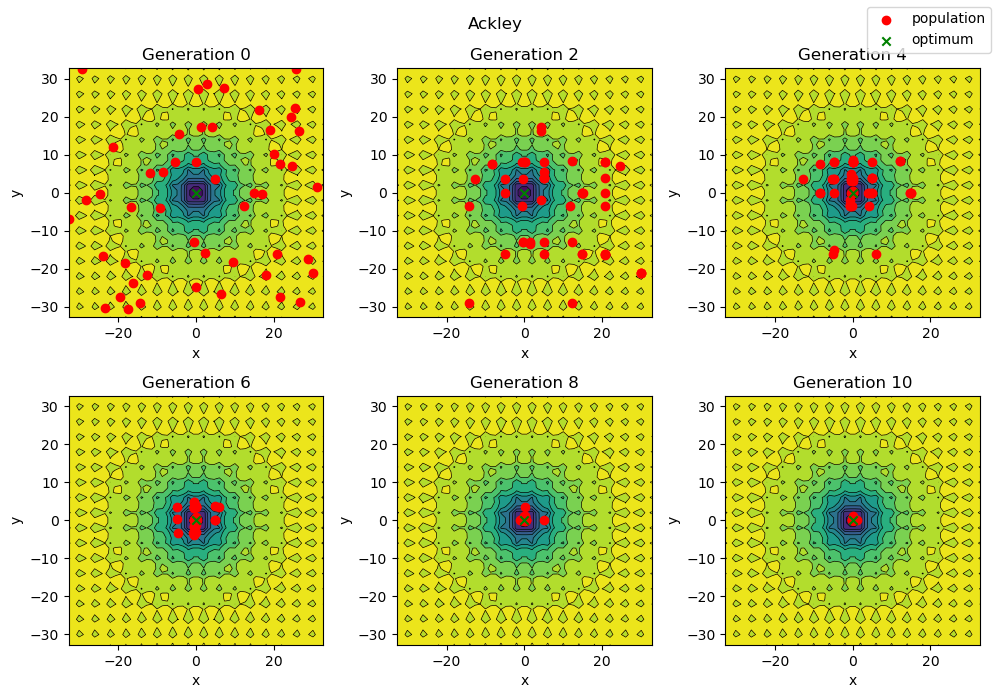
\includegraphics[width=\textwidth]{lab7/imgs/ga_ackley.png}
        \caption{Ackley function}
    \end{subfigure}
    \begin{subfigure}{0.5\textwidth}
        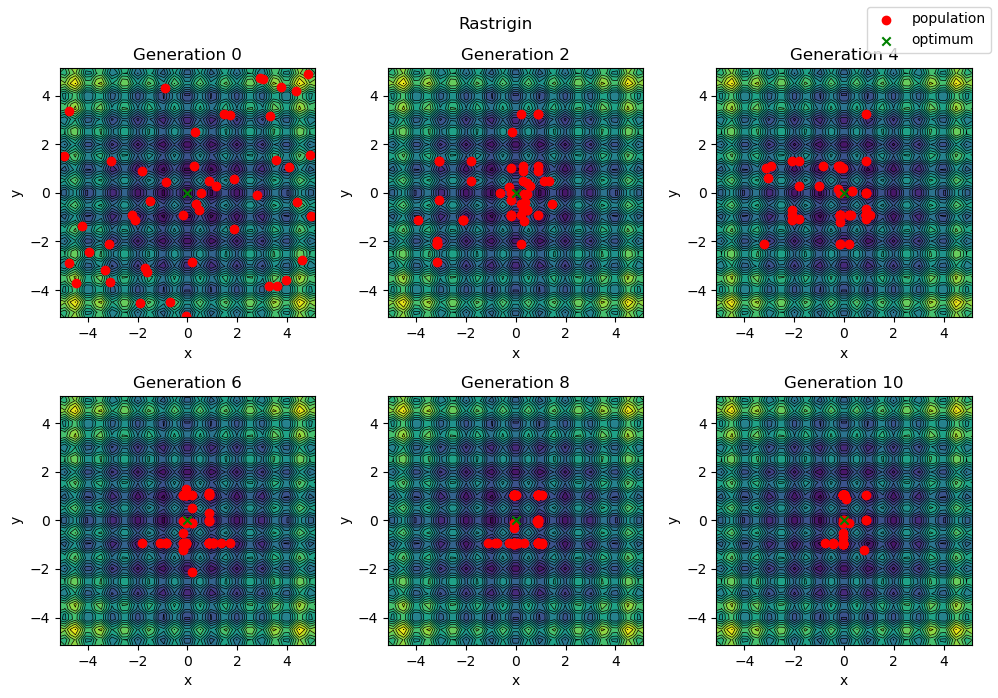
\includegraphics[width=\textwidth]{lab7/imgs/ga_rastrigin.png}
        \caption{Rastringin function}
    \end{subfigure}\\
    \begin{subfigure}{0.5\textwidth}
        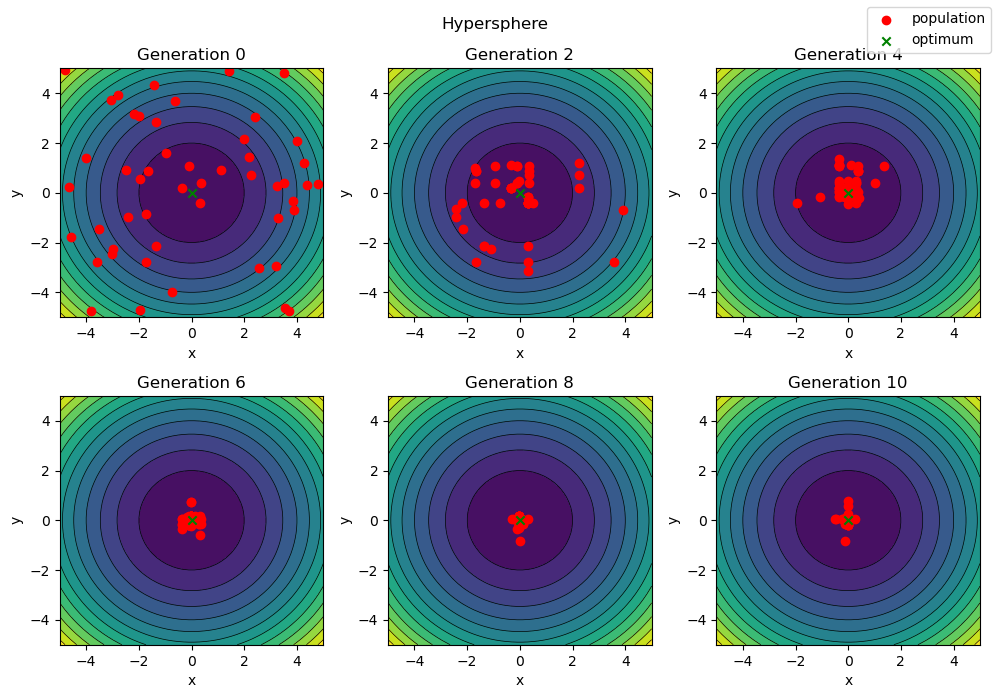
\includegraphics[width=\textwidth]{lab7/imgs/ga_hypersphere.png}
        \caption{Hypersphere function}
    \end{subfigure}
    \begin{subfigure}{0.5\textwidth}
        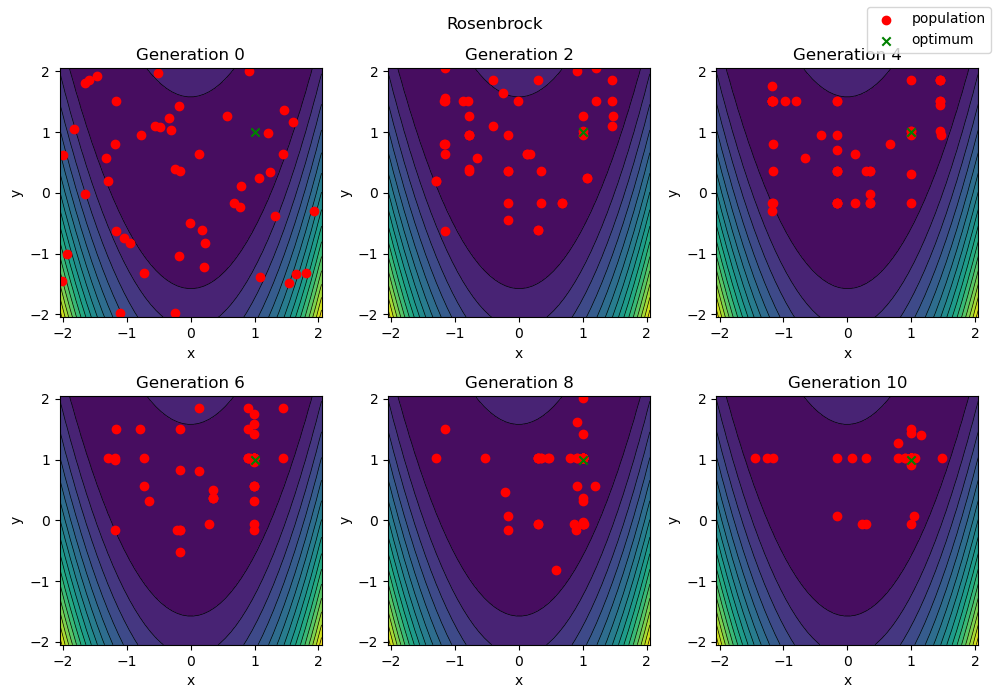
\includegraphics[width=\textwidth]{lab7/imgs/ga_rosenbrock.png}
        \caption{Rosenbrock function}
    \end{subfigure}
    \caption{Comparison of different objective functions for the GA algorithm}
    \label{fig:ga-comp}
\end{figure}



\subsection{Evolution Strategies}
Evolution Strategies are a class of metaheuristics that are similar to genetic algorithms that evolve the mutation rate together with the solution.

Unless specified, the following parameters are used:
\begin{itemize}
    \item Population size: 50
    \item Number of generations: 50
    \item Objective function: Ackley
    \item Strategy: None
    \item Number of simulations: 10
\end{itemize}

\paragraph*{Offspring size}
We can see that the performance of the algorithm is better for larger offspring sizes. This is because the algorithm is able to explore the search space better but with the tradeoff of computational complexity. The results are shown in Table \ref{tab:es-offspring_size}.
\begin{table}[H]
    \centering
    \begin{tabular}{|c|c|c|}
        Offspring size & Average fitness & Standard deviation \\ \hline
        50             & 0.0920          & 0.0699             \\
        100            & 0.0787          & 0.0303             \\
        200            & 0.0325          & 0.0238             \\
        300            & 0.0236          & 0.0099             \\
        400            & 0.0104          & 0.0108             \\
        500            & 0.0282          & 0.0131             \\
    \end{tabular}
    \caption{Different offspring sizes with mutation rate 0.2}
    \label{tab:es-offspring_size}
\end{table}

\paragraph*{Strategy}
We now test different strategy to evolve the mutation rate:
\begin{itemize}
    \item None: the mutation rate is fixed
    \item Global: each individual evolves a single mutation rate (sphere)
    \item Individual: each individual has a mutation rate for each gene / dimension (axis-parallel ellipsoid)
    \item Correlated: each individual has a mutation rate for each gene and the interaction between every pair of genes (general ellipsoid)
\end{itemize}
We can see that the best performance is obtained with the global strategy probably because there is no skewed narrow valley to be found in the Ackley function that would require a more complex strategy. The results are shown in Table \ref{tab:es-strategy}.
\begin{table}[H]
    \centering
    \begin{tabular}{|c|c|c|}
        Strategy   & Average fitness & Standard deviation \\ \hline
        None       & 4.57e-02        & 1.91e-02           \\
        Global     & 1.41e-06        & 4.09e-07           \\
        Individual & 1.75e-04        & 2.51e-04           \\
        Correlated & 6.38e-02        & 1.10e-01           \\
    \end{tabular}
    \caption{Different strategies with offspring size 100}
    \label{tab:es-strategy}
\end{table}

\subsection{Particle Swarm Optimization}
Particle Swarm Optimization is a population-based optimization technique that is inspired by the social behavior of flocks of birds. The algorithms aims at finding emerging social behaviours starting from few simple local rules. These rules are:
\begin{itemize}
    \item each position in the environment is associated with a reward
    \item each particle has memory of the best position it visited
    \item each particle gets information from its neighbours
\end{itemize}

\paragraph*{Population size / Generation ratio}
We compare the performances of the algorithm by changing the number of individuals in the population and the number of generations but keeping the ratio constant (so to have the same number of evaluations). We can see that the performance is better for larger populations and smaller number of generations. The results are shown in Table \ref{tab:pso-pop-gen}.
\begin{table}[H]
    \centering
    \begin{tabular}{|c|c|c|c|}
        Population size & Generations & Average fitness & Standard deviation \\ \hline
        20              & 125         & 7.99e-16        & 1.74e-15           \\
        40              & 62          & 1.02e-11        & 5.92e.12           \\
        60              & 41          & 7.53e-08        & 3.05e-08           \\
        80              & 31          & 4.30e-06        & 1.99e-06           \\
        100             & 25          & 4.05e-05        & 4.05e-05           \\
    \end{tabular}
    \caption{Different population sizes and generation numbers with mutation rate 0.2}
    \label{tab:pso-pop-gen}
\end{table}

\paragraph*{Topology}
We now test different topologies for the algorithm:
\begin{itemize}
    \item Ring: each particle gets information from the N closest particles
    \item Star: each particle gets information from all other particles
\end{itemize}
The best performances are obtained by the star topology because the each particle gets information by a larger number of particles. To confirm this trend, we can see that the performance of the ring topology increases with the number of neighbours. The results are shown in Table \ref{tab:pso-topology}.
\begin{table}[H]
    \centering
    \begin{tabular}{|c|c|c|}
        Topology & Average fitness & Standard deviation \\ \hline
        Star     & 1.62e-09        & 1.16e-09           \\
        Ring 2   & 4.58e-04        & 3.67e-04           \\
        Ring 5   & 2.37e-07        & 3.24e-07           \\
        Ring 10  & 1-90e-08        & 2.31e-08           \\
        Ring 20  & 4.22e-09        & 2.24e-09           \\
        Ring 30  & 3.18e-09        & 1.97e-09           \\
        Ring 40  & 2.80e-09        & 1.71e-09           \\
    \end{tabular}
    \caption{Different topologies with population size 40 and generation number 62}
    \label{tab:pso-topology}
\end{table}